% ===== handout mode =====
% Comment/uncomment this line to toggle handout mode
% \newcommand{\handout}{}

% Comment/uncoment this line to toogle Mortitz mode
% \newcommand{\Moritz}{}

% Comment/uncomment this line to toggle handout mode
% \newcommand{\handout}{}

% by Stephan

%% Moritz mode or Stephan mode
\ifdefined \MoritzMode

% This is a configuration file with private, tutor specific information.
% It is therefore excluded from the Git repository so changes in this file will not conflict in git commits.

% Copy this Template, rename to config.tex and add your information below.

\newcommand{\mymail}{moritz.laupichler@student.kit.edu} % Consider using your named student Mail address to keep your u-Account private.

\newcommand{\myname}{\href{mailto:\mymail}{Moritz Laupichler}}

\newcommand{\mytutnumber}{27}

\newcommand{\mytutinfos}{Dienstags, 5. Block (15:45-17:15), SR 236}

\newcommand{\aboutMeFrame}{
	\begin{frame}{Euer Tutor}
		Name: \myname \\
		Alter: 19 Jahre \\
		Studiengang: Bachelor Informatik, 3. Semester \\
		\vspace{1cm}
		\pause 
		\centering{Kontakt: \href{mailto:\mymail}{\mymail}}
	\end{frame}
}

% Toggle Handout mode by including the following line before including style_tut
% and removing the % at the start (but do NOT remove it here, otherwise handout mode will always be on!)
% Please keep handout mode on in all commits!

% \newcommand{\handout}{} % Moritz mode
\fi
\ifdefined \AlexMode

% This is a configuration file with private, tutor specific information.
% It is therefore excluded from the Git repository so changes in this file will not conflict in git commits.

% Copy this Template, rename to config.tex and add your information below.

\newcommand{\mymail}{alexander.klug@student.kit.edu} % Consider using your named student Mail address to keep your u-Account private.

\newcommand{\myname}{\href{mailto:\mymail}{Alexander Klug}}

\newcommand{\mytutnumber}{30}

\newcommand{\mytutinfos}{Mittwochs, 3. Block (11:30-13:00), SR -107}

\newcommand{\aboutMeFrame}{
	\begin{frame}{Euer Tutor}
		Name: \myname \\
		Alter: 19 Jahre \\
		Studiengang: Bachelor Informatik, 3. Semester \\
		\vspace{1cm}
		\pause 
		\centering{Kontakt: \href{mailto:\mymail}{\mymail}}
	\end{frame}
}

% Toggle Handout mode by including the following line before including style_tut
% and removing the % at the start (but do NOT remove it here, otherwise handout mode will always be on!)
% Please keep handout mode on in all commits!

% \newcommand{\handout}{} % Alex Mode
\fi
\ifdefined \StephanMode

% This is a configuration file with private, tutor specific information.
% It is therefore excluded from the Git repository so changes in this file will not conflict in git commits.

% Copy this Template, rename to config.tex and add your information below.

\newcommand{\mymail}{stephan.bohr@student.kit.edu} % Consider using your named student Mail address to keep your u-Account private.

\newcommand{\myname}{\href{mailto:\mymail}{Stephan Bohr}}

\newcommand{\mytutnumber}{19}

\newcommand{\mytutinfos}{Dienstags, 3. Block (11:30-13:00), SR -108}

\newcommand{\aboutMeFrame}{
	\begin{frame}{Euer Tutor}
		Name: \myname \\
		Alter: 21 Jahre \\
		Studiengang: Bachelor Informatik, 5. Semester \\
		\vspace{1cm}
		\pause 
		\centering{Kontakt: \href{mailto:\mymail}{\mymail}}
	\end{frame}
} % Stephan mode
\fi

%% Beamer-Klasse im korrekten Modus
\ifdefined \handout
\documentclass[handout]{beamer} % Handout mode
\else
\documentclass{beamer}
\fi
%\documentclass[18pt,parskip]{beamer}

%% SLIDE FORMAT

% use 'beamerthemekit' for standard 4:3 ratio
% for widescreen slides (16:9), use 'beamerthemekitwide'

\usepackage{../templates/KIT-slides/beamerthemekit}
%\usepackage{../templates/KIT-slides/beamerthemekitwide}

%% TITLE PICTURE

% if a custom picture is to be used on the title page, copy it into the 'logos'
% directory, in the line below, replace 'mypicture' with the 
% filename (without extension) and uncomment the following line
% (picture proportions: 63 : 20 for standard, 169 : 40 for wide
% *.eps format if you use latex+dvips+ps2pdf, 
% *.jpg/*.png/*.pdf if you use pdflatex)

\titleimage{../figures/titleimage/brain}

%% TITLE LOGO

% for a custom logo on the front page, copy your file into the 'logos'
% directory, insert the filename in the line below and uncomment it

%\titlelogo{mylogo}

% (*.eps format if you use latex+dvips+ps2pdf,
% *.jpg/*.png/*.pdf if you use pdflatex)

%% TikZ INTEGRATION

% use these packages for PCM symbols and UML classes
% \usepackage{templates/tikzkit}
% \usepackage{templates/tikzuml}

%\usepackage{tikz}
%\usetikzlibrary{matrix}
%\usetikzlibrary{arrows.meta}
%\usetikzlibrary{automata}
%\usetikzlibrary{tikzmark}

%%%%%%%%%%%%%%%%%%%%%%%%%
% Libertine font (Original GBI font)
\usepackage[mono=false]{libertine}
%\renewcommand*\familydefault{\sfdefault}  %% Only if the base font of the document is to be sans serif

%% Schönere Schriften
\usepackage[TS1,T1]{fontenc}

%% Deutsche Silbentrennung und Beschriftungen
\usepackage[ngerman]{babel}

%% UTF-8-Encoding
\usepackage[utf8]{inputenc}

%% Bibliotheken für viele mathematische Symbole
\usepackage{amsmath, amsfonts, amssymb}

%% Anzeigetiefe für Inhaltsverzeichnis: 1 Stufe
\setcounter{tocdepth}{1}

%% Hyperlinks
\usepackage{hyperref}
% I don't know why, but this works and only includes sections and NOT subsections in the pdf-bookmarks.
\hypersetup{bookmarksdepth=subsection}

%% remove navigation symbols
\setbeamertemplate{navigation symbols}{}

%% switch between "ngerman" and "english" for German/English style date and logos
\selectlanguage{ngerman}

%% for invisible pause texts instead of dimming
\setbeamercovered{invisible}

\usepackage[german=swiss]{csquotes}

\usepackage{tabularx}
\usepackage{booktabs}

\usepackage{tikz}


% Problem: disabled itemize-icons
%\usepackage{enumitem}
% %\setlist[enumerate]{topsep=0pt,itemsep=-1ex,partopsep=1ex,parsep=1ex}
% \setlist[itemize]{noitemsep, nolistsep}
% \setlist[enumerate]{noitemsep, nolistsep}

% Mathmode no vertical space (https://tex.stackexchange.com/a/47403/146825)
\setlength{\abovedisplayskip}{0pt}
\setlength{\belowdisplayskip}{0pt}
\setlength{\abovedisplayshortskip}{0pt}
\setlength{\belowdisplayshortskip}{0pt}

%%%%%%%%%%%% Slides %%%%%%%%%%%%%%%%

\newcommand{\Moritz}[1]{
	\ifdefined \MoritzMode
	#1
	\fi
}

\newcommand{\Alex}[1]{
	\ifdefined \AlexMode
	#1
	\fi
}

\newcommand{\Stephan}[1]{
	\ifdefined \StephanMode
	#1
	\fi
}

\newcommand{\notMoritz}[1]{
	\Alex{#1} \Stephan{#1}
}

\newcommand{\notAlex}[1]{
	\Moritz{#1} \Stephan{#1}
}

\newcommand{\notStephan}[1]{
	\Alex{#1} \Moritz{#1}
}

%% Wochennummer
%\newcounter{weeknum}

%% Titelinformationen
%\title[GBI Tutorium, Woche \theweeknum]{Grundbegriffe der Informatik \\ Tutorium \mytutnumber}
%\subtitle{Termin \theweeknum \ | \mydate \\ \myname}
\author[\myname]{\myname}
\institute{Fakultät für Informatik}
%\date{\mydate}

%% Titel einfügen
\newcommand{\titleframe}{\frame{\titlepage}\addtocounter{framenumber}{-1}}


%% Alles starten mit \starttut{X}
%\newcommand{\starttut}[1]{\setcounter{weeknum}{#1}\titleframe\frame{\frametitle{Inhalt}\tableofcontents} \AtBeginSection[]{%
%\begin{frame}
%	\tableofcontents[currentsection]
%\end{frame}\addtocounter{framenumber}{-1}}}


%\newcommand{\framePrevEpisode}{
%	\begin{frame}
%		\centering
%		\textbf{In the previous episode of GBI...}
%	\end{frame}
%}

%% Roadmap frame
%table of contents
\newcommand{\roadmap}{
	\frame{\frametitle{Roadmap}\tableofcontents}}

 \AtBeginSection[]{%
\begin{frame}
	\frametitle{Roadmap}
	\tableofcontents[currentsection]
\end{frame}%\addtocounter{framenumber}{-1}
}


%% ShowMessage frame
\newcommand{\showmessage}[1]{\frame{\frametitle{\phantom{1em}}\centering\textbf{#1}}}

%% Fragen
%% Lastframe
\newcommand{\questionframe}{\showmessage{Fragen?}}

%% Lastframe
\newcommand{\lastframe}{\showmessage{Vielen Dank für Eure Aufmerksamkeit! \\Bis nächste Woche :)}}

%% Thanks frame
\newcommand{\slideThanks}{
	\begin{frame}
		\frametitle{Credits}
		\begin{block}{}
			An der Erstellung des Foliensatzes haben mitgewirkt:\\[1em]
			\Moritz{
			Stephan Bohr \\
			Alexander Klug \\
			}
			\Alex{
			Stephan Bohr \\
			Moritz Laupichler \\
			}
			\Stephan{
			Moritz Laupichler \\
			Alexander Klug \\
			}
			Katharina Wurz \\
			Thassilo Helmold \\
			Daniel Jungkind \\
			% Philipp Basler \\
			% Nils Braun \\
			% Dominik Doerner \\
			% Ou Yue \\
		\end{block}
	\end{frame}
}

%% Verbatim
%\usepackage{moreverb}

% GBI related stuff, but not beamer-stuff
\newcommand{\newpar}[1]{\paragraph{#1}\mbox{}\newline}

\newcommand{\nM}{\mathbb{M}}
\newcommand{\nR}{\mathbb{R}}
\newcommand{\nN}{\mathbb{N}}
\newcommand{\nZ}{\mathbb{Z}}
\newcommand{\nQ}{\mathbb{Q}}
\newcommand{\nB}{\mathbb{B}}
\newcommand{\nC}{\mathbb{C}}
\newcommand{\nK}{\mathbb{K}}
\newcommand{\nF}{\mathbb{F}}
\newcommand{\nG}{\mathbb{G}}
\newcommand{\nullel}{\mathcal{O}}
\newcommand{\einsel}{\mathds{1}}
\newcommand{\nP}{\mathbb{P}}
\newcommand{\Pot}{\mathcal{P}}
\renewcommand{\O}{\text{O}}

\newcommand{\bfmod}{\ensuremath{\text{\textbf{ mod }}}}
\renewcommand{\mod}{\bfmod}
\newcommand{\bfdiv}{\ensuremath{\text{\textbf{ div }}}}
\renewcommand{\div}{\bfdiv}


\newcommand{\set}[1]{\left\{ #1 \right\}}
\newcommand{\setc}[2]{\set{#1 \mid #2}}
\newcommand{\setC}[2]{\set{#1 \mid \text{ #2 }}}

\newcommand{\setsize}[1]{\; \mid #1 \mid \; }

\newcommand{\q}[1]{\textquotedblleft #1\textquotedblright}

% Zu zeigen, thx to http://www.matheboard.de/archive/155832/thread.html
\newcommand{\zz}{\ensuremath{\mathrm{z\kern-.29em\raise-0.44ex\hbox{z}}}:}

% Text above symbol
% https://tex.stackexchange.com/a/74132/146825
%
% \newcommand{\eqtext}[1]{\stackrel{\mathclap{\normalfont\mbox{#1}}}{=}}
% \newcommand{\gdwtext}[1]{\stackrel{\mathclap{\normalfont\mbox{#1}}}{\Leftrightarrow}}
% \newcommand{\imptext}[1]{\stackrel{\mathclap{\normalfont\mbox{#1}}}{\Rightarrow}}
% \newcommand{\symbtext}[2]{\stackrel{\mathclap{\normalfont\mbox{#2}}}{#1}}
\newcommand{\eqtext}[1]{\mathrel{\overset{\makebox%[0pt]
{\mbox{\normalfont\tiny #1}}}{=}}}
\newcommand{\gdwtext}[1]{\mathrel{\overset{\makebox%[0pt]
{\mbox{\normalfont\tiny #1}}}{\ensuremath{\Leftrightarrow}}}}
\newcommand{\imptext}[1]{\mathrel{\overset{\makebox%[0pt]
{\mbox{\normalfont\tiny #1}}}{\ensuremath{\Rightarrow}}}}
\newcommand{\symbtext}[2]{\mathrel{\overset{\makebox%[0pt]
{\mbox{\normalfont\tiny #2}}}{#1}}}

% qed symbol
\newcommand{\qedblack}{\hfill \ensuremath{\blacksquare}}
\newcommand{\qedwhite}{\hfill \ensuremath{\Box}}

% Aussagenlogik
% Worsch
\colorlet{alcolor}{blue}
\RequirePackage{tikz}
\usetikzlibrary{arrows.meta}
\newcommand{\alimpl}{\mathrel{\tikz[x={(0.1ex,0ex)},y={(0ex,0.1ex)},>={Classical TikZ Rightarrow[]}]{\draw[alcolor,->,line width=0.7pt,line cap=round] (0,0) -- (15,0);\path (0,-6);}}}
\newcommand{\alimp}{\alimpl}
\newcommand{\aleqv}{\mathrel{\tikz[x={(0.1ex,0ex)},y={(0ex,0.1ex)},>={Classical TikZ Rightarrow[]}]{\draw[alcolor,<->,line width=0.7pt,line cap=round] (0,0) -- (18,0);\path (0,-6);}}}
\newcommand{\aland}{\mathbin{\raisebox{-0.6pt}{\rotatebox{90}{\texttt{\color{alcolor}\char62}}}}}
\newcommand{\alor}{\mathbin{\raisebox{-0.8pt}{\rotatebox{90}{\texttt{\color{alcolor}\char60}}}}}
%\newcommand{\ali}[1]{_{\mathtt{\color{alcolor}#1}}}
\newcommand{\alv}[1]{\mathtt{\color{alcolor}#1}}
\newcommand{\alnot}{\mathop{\tikz[x={(0.1ex,0ex)},y={(0ex,0.1ex)}]{\draw[alcolor,line width=0.7pt,line cap=round,line join=round] (0,0) -- (10,0) -- (10,-4);\path (0,-8) ;}}}
\newcommand{\alP}{\alv{P}} %ali{#1}}
%\newcommand{\alka}{\negthinspace\hbox{\texttt{\color{alcolor}(}}}
\newcommand{\alka}{\negthinspace\text{\texttt{\color{alcolor}(}}}
%\newcommand{\alkz}{\texttt{\color{alcolor})}}\negthinspace}
\newcommand{\alkz}{\text{\texttt{\color{alcolor})}}\negthinspace}

% Thassilo
\newcommand{\BB}{\mathbb{B}}
\newcommand{\boder}{\alor}%{\ensuremath{\text{\;}\textcolor{blue}{\vee}}\text{\;}}
\newcommand{\bund}{\aland}%{\ensuremath{\text{\;}\textcolor{blue}{\wedge}}\text{\;}}
\newcommand{\bimp}{\alimp}%{\ensuremath{\text{\;}\textcolor{blue}{\to}}\text{\;}}
\newcommand{\bnot}{\alnot}%{\ensuremath{\text{\;}\textcolor{blue}{\neg}}\text{}}
\newcommand{\bgdw}{\aleqv}%{\ensuremath{\text{\;}\textcolor{blue}{\leftrightarrow}}\text{\;}}
\newcommand{\bone}{\ensuremath{\textcolor{blue}{1}}\text{}}
\newcommand{\bzero}{\ensuremath{\textcolor{blue}{0}}\text{}}
\newcommand{\bleftBr}{\alka}%{\ensuremath{\textcolor{blue}{(}}\text{}}
\newcommand{\brightBr}{\alkz}%{\ensuremath{\textcolor{blue}{)}}\text{}}

\newcommand{\val}{\hbox{\textit{val}}}

\newcommand{\VarAL}{\hbox{\textit{Var}}_{AL}}
\newcommand{\ForAL}{\hbox{\textit{For}}_{AL}}

% Validierungsfunktion val_i
\newcommand{\vali}[1]{\ensuremath{\val_I(#1)}}

% Boolsche Funktion b_
\newcommand{\bfnot}[1]{\ensuremath{b_{\bnot}(#1)}}
\newcommand{\bfand}[2]{\ensuremath{b_{\bund}(#1,#2)}}
\newcommand{\bfor}[2]{\ensuremath{b_{\boder}(#1,#2)}}
\newcommand{\bfimp}[2]{\ensuremath{b_{\bimp}(#1,#2)}}

% Aussagenkalkül
\newcommand{\AAL}{A_{AL}}
\newcommand{\LAL}{\hbox{\textit{For}}_{AL}}
\newcommand{\AxAL}{\hbox{\textit{Ax}}_{AL}}
\newcommand{\MP}{\hbox{\textit{MP}}}

% Prädikatenlogik
% die nachfolgenden Sachen angepasst an cmtt
\newlength{\ttquantwd}
\setlength{\ttquantwd}{1ex}
\newlength{\ttquantht}
\setlength{\ttquantht}{6.75pt}
\def\plall{%
  \tikz[line width=0.67pt,line cap=round,line join=round,baseline=(B),alcolor] {
    \draw (-0.5\ttquantwd,\ttquantht) -- node[coordinate,pos=0.4] (lll){} (-0.25pt,-0.0pt) -- (0.25pt,-0.0pt) -- node[coordinate,pos=0.6] (rrr){} (0.5\ttquantwd,\ttquantht);
    \draw (lll) -- (rrr);
    \coordinate (B) at (0,-0.35pt);
  }%
}
\def\plexist{%
  \tikz[line width=0.67pt,line cap=round,line join=round,baseline=(B),alcolor] {
    \draw (-0.9\ttquantwd,\ttquantht) -- (0,\ttquantht) -- node[coordinate,pos=0.5] (mmm){} (0,0) --  (-0.9\ttquantwd,0);
    \draw (mmm) -- ++(-0.75\ttquantwd,0);
    \coordinate (B) at (0,-0.35pt);
  }\ensuremath{\,}%
}
\let\plexists=\plexist
\newcommand{\NT}[1]{\ensuremath{\langle\mathrm{#1} \rangle}}
\newcommand{\CPL}{\text{\itshape Const}_{PL}}
\newcommand{\FPL}{\text{\itshape Fun}_{PL}}
\newcommand{\RPL}{\text{\itshape Rel}_{PL}}
\newcommand{\VPL}{\text{\itshape Var}_{PL}}
\newcommand{\plka}{\alka}
\newcommand{\plkz}{\alkz}
%\newcommand{\plka}{\plfoo{(}}
%\newcommand{\plkz}{\plfoo{)}}
\newcommand{\plcomma}{\hbox{\texttt{\color{alcolor},}}}
\newcommand{\pleq}{{\color{alcolor}\,\dot=\,}}

\newcommand{\plfoo}[1]{\mathtt{\color{alcolor}#1}}
\newcommand{\plc}{\plfoo{c}}
\newcommand{\pld}{\plfoo{d}}
\newcommand{\plf}{\plfoo{f}}
\newcommand{\plg}{\plfoo{g}}
\newcommand{\plh}{\plfoo{h}}
\newcommand{\plx}{\plfoo{x}}
\newcommand{\ply}{\plfoo{y}}
\newcommand{\plz}{\plfoo{z}}
\newcommand{\plR}{\plfoo{R}}
\newcommand{\plS}{\plfoo{S}}
\newcommand{\ar}{\mathrm{ar}}

\newcommand{\bv}{\mathrm{bv}}
\newcommand{\fv}{\mathrm{fv}}

\def\word#1{\hbox{\textcolor{blue}{\texttt{#1}}}}
%\let\literal\word
\def\mword#1{\hbox{\textcolor{blue}{$\mathtt{#1}$}}}  % math word
\def\sp{\scalebox{1}[.5]{\textvisiblespace}}
\def\wordsp{\word{\sp}}


\newcommand{\W}{\ensuremath{\hbox{\textbf{w}}}\xspace}
\newcommand{\F}{\ensuremath{\hbox{\textbf{f}}}\xspace}
\newcommand{\WF}{\ensuremath{\{\W,\F\}}\xspace}
\newcommand{\valDIb}{\val_{D,I,\beta}}

\newcommand{\impl}{\ifmmode\ensuremath{\mskip\thinmuskip\Rightarrow\mskip\thinmuskip}\else$\Rightarrow$\fi\xspace}
\newcommand{\Impl}{\ifmmode\implies\else$\Longrightarrow$\fi\xspace}

\newcommand{\derives}{\Rightarrow}

\newcommand{\gdw}{\ifmmode\mskip\thickmuskip\Leftrightarrow\mskip\thickmuskip\else$\Leftrightarrow$\fi\xspace}
\newcommand{\Gdw}{\ifmmode\iff\else$\Longleftrightarrow$\fi\xspace}

\newcommand*{\from}{\colon}
\newcommand{\functionto}{\longrightarrow}


\newcommand{\LTer}{L_{\text{\itshape Ter}}}
\newcommand{\LRel}{L_{\text{\itshape Rel}}}
\newcommand{\LFor}{L_{\text{\itshape For}}}
\newcommand{\NTer}{N_{\text{\itshape Ter}}}
\newcommand{\NRel}{N_{\text{\itshape Rel}}}
\newcommand{\NFor}{N_{\text{\itshape For}}}
\newcommand{\PTer}{P_{\text{\itshape Ter}}}
\newcommand{\PRel}{P_{\text{\itshape Rel}}}
\newcommand{\PFor}{P_{\text{\itshape For}}}

\newcommand{\sgn}{\mathop{\text{sgn}}}

\newcommand{\lang}[1]{\ensuremath{\langle#1\rangle}}

\newcommand{\literal}[1]{\hbox{\textcolor{blue!95!white}{\textup{\texttt{\scalebox{1.11}{#1}}}}}}
\let\hashtag\#
\renewcommand{\#}[1]{\literal{#1}}

\def\blank{\ensuremath{\openbox}}
\def\9{\blank}
\newcommand{\io}{\!\mid\!}


\providecommand{\fspace}{\mathord{\text{space}}}
\providecommand{\fSpace}{\mathord{\text{Space}}}
\providecommand{\ftime}{\mathord{\text{time}}}
\providecommand{\fTime}{\mathord{\text{Time}}}

\newcommand{\fnum}{\text{num}}
\newcommand{\fNum}{{\text{Num}}}

\def\Pclass{\text{\bfseries P}}
\def\PSPACE{\text{\bfseries PSPACE}}



\title[Formale Sprachen, Aussagenlogik]{2. Tutorium\\ Formale Sprachen, Aussagenlogik}
\subtitle{Grundbegriffe der Informatik, Tutorium \hashtag\mytutnumber}
\date{\today}

\begin{document}
\titleframe
\roadmap

\section{Organisatorisches}
\subsection{Tipps}
\begin{frame}{Allgemeine Tipps}
    \begin{itemize}[<+->]
    	\item Jedes abgegebene Blatt: \emph{Kopfzeile} mit \\{\centering``GBI ÜB 1, \quad Tut. \hashtag\mytutnumber\ (Tutorname), \quad Max Mustermann, 1234567''}
    	% \item Aufgabenblatt muss \emph{nicht ausgedruckt} werden
		% \item Kein Bleistift,
        \item Kein roter oder grüner Stift
		\item Achtet auf die \emph{Aufgabenstellung}: Unterschied  ``Gib an'', ``Beweise'' oder ``Begründe''
		\item Bei Beweis \alert{NIEMALS} Beispiel, Widerlegen oft einfaches Gegenbeispiel
		\item Gebt nur \emph{eine Version} an, sonst bewerte ich die schlechtere
    	\end{itemize}
\end{frame}

\begin{frame}{Allgemeine Tipps}
    \begin{itemize}[<+->]
    	\item \emph{Strukturiert vorgehen!} Schreibt ``Beh.:'', ``\zz'', ``Ann.:'',\\
    	setzt ``q.e.d oder $\qedsymbol$'' ans Ende eines Beweises
    	\item \emph{Führt den Leser} bei Beweisen, macht klar, was ihr meint, was ihr in einem Schritt tut
    	\item Formalisiert so viel wie nötig, aber nicht mehr
    	\item Neue Definitionen mit \emph{$:=$}, z.B. $A_n := c^2$
    	\item \emph{Funktionen vollständig} angeben: $f \from \nN_0 \to \nR, x \mapsto x^2$ o.ä.
    \end{itemize}
\end{frame}
\subsection{UB1}
\Kilian{}
\Moritz{}
\Stephan{
\begin{frame}{Zum ersten Übungsblatt}
    \begin{itemize}
    	\item Unterschied $\cup$ und $\vee$
    	\item Aufgabe mit $A \subseteq B \subseteq C$ war keine Abbildung
    	\item[]
    	\item Im Durchschnitt 88,24 \%
    \end{itemize}
\end{frame}
}

\Stephan{
\section[Relationen (Wdh.)]{Wiederholung: Relationen}
\begin{frame}{Relationen und Abbildungen}
	\begin{exampleblock}{Beispiel \hashtag2}
		\begin{minipage}{0.5\textwidth}
			\begin{tikzpicture}
			[scale=0.6,auto=left,every node/.style={circle,fill=kit-blue30}]
			\node (a1) at (0,10)  {$a_1$};
			\node (a2) at (0,8)  {$a_2$};
			% \node (a3) at (0,6)  {$a_3$};
			\node (b1) at (2,10)  {$b_1$};
			\node (b2) at (2,8)  {$b_2$};
			\node (b3) at (2,6)  {$b_3$};
			
			
			\foreach \from/\to in {a1/b2, a2/b3, a2/b1}
			\draw (\from) -- (\to);
			\end{tikzpicture}
		\end{minipage} \hfill
		\begin{minipage}{0.45\textwidth}
			\raggedright
			% \begin{align*}
			% Linkstotal&: \only<2->{Ja} \\
			% Rechtseindeutig&: \only<3->{Nein} \\
			% Rechtstotal bzw. surjektiv&: \only<4->{Nein} \\
			% Linkseindeutig bzw. injektiv&: \only<5->{Nein} \\
			% \end{align*}
			\begin{tabular}{rl}
			Linkstotal: & \only<2->{\textcolor{kit-green100}{Ja}} \\
			Rechtseindeutig: & \only<3->{\textcolor{kit-red100}{Nein}}\\ 
			Rechtstotal: & \only<4->{\textcolor{kit-green100}{Ja}} \\
			Linkseindeutig: & \only<5->{\textcolor{kit-green100}{Ja}} \\
			Bijektive Abbildung: & \only<6->{\textcolor{kit-red100}{Nein}} \\
			\only<7->{Abbildung: }& \only<7->{\textcolor{kit-red100}{Nein}}
			\end{tabular}

		\end{minipage}
	\end{exampleblock}
\end{frame}
	\subsection{Aufgabe}
\begin{frame}{Aufgabe}
\begin{figure}[h!]
		\centering
		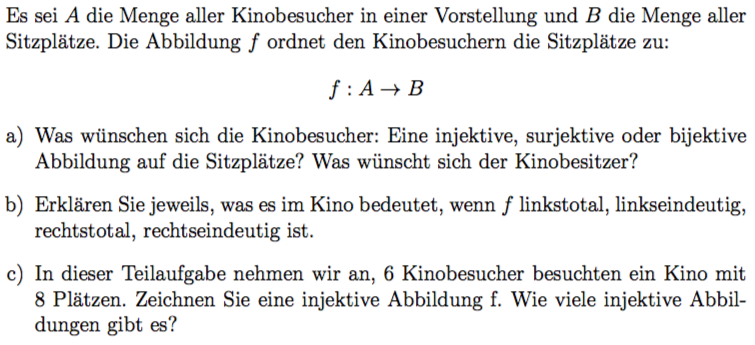
\includegraphics[width=\textwidth]{../topics/mengen-relationen-abbildungen/1.png} 
	\end{figure}     
\end{frame}

\begin{frame}{Aufgabe}
\begin{figure}[h!]
		\centering
		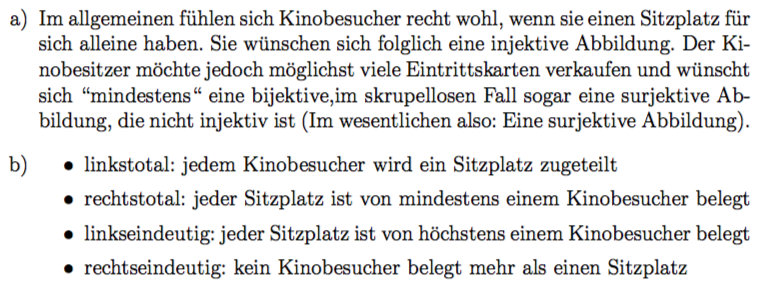
\includegraphics[width=\textwidth]{../topics/mengen-relationen-abbildungen/2.png} 
	\end{figure}  
	\begin{figure}[h!]
		\centering
		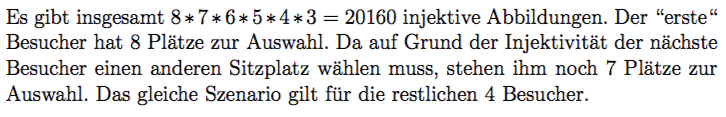
\includegraphics[width=\textwidth]{../topics/mengen-relationen-abbildungen/3.png} 
	\end{figure}   
\end{frame}		
}

\section{Formale Sprachen}
\subsection{Alphabete, Wörter, Sprachen}
\begin{frame}{Alphabete, Wörter, Sprachen}
	\begin{block}{Def.: Alphabet}
		Ein \textbf{Alphabet} ist eine endliche, nichtleere Menge von Zeichen.
	\end{block}
	\pause
	\begin{block}{Def.: Wort}
		Ein \textbf{Wort} über einem Alphabet A ist eine Folge von Zeichen aus A.
	\end{block}
	\pause
	\begin{block}{Def.: leeres Wort}
		Das \textbf{leere Wort} \(\varepsilon\) ist das Wort, das aus null Zeichen besteht, d.h. es hat die Länge 0.
	\end{block}
\end{frame}

\begin{frame}{Alphabete, Wörter, Sprachen}
	\begin{block}{Def.: Wort (formell)}
		Ein \textbf{Wort} $w$ über einem Alphabet $A$ ist eine surjektive Abbildung $w \from \nZ_n \to B \subseteq A$ mit $\nZ_n := \setc{i \in \nN_0}{0 \le i < n}$.
	\end{block}

	\begin{block}{Def.: leeres Wort (formell)}
		Das \textbf{leere Wort} $\varepsilon$ ist die Abbildung $\varepsilon \from \nZ_0 = \set{} \to \set{}$.	
	\end{block}

	\begin{alertblock}{Beachte}
		$\set{\varepsilon} \neq \emptyset$	
	\end{alertblock}

\end{frame}

\begin{frame}{Alphabete, Wörter, Sprachen}
	\begin{block}{Def.: \(A^{n}\)}
		\textbf{\(A^{n}\)} ist die Menge aller Wörter der Länge n über dem Alphabet A.
	\end{block}
	\pause
	\begin{block}{Def.: \(A^{*}\)}
		\textbf{\(A^{*}\)} ist die Menge aller Wörter beliebiger Länge über dem Alphabet A.		
		\[
			A^{*}= \bigcup_{i=0}^{\infty} A^{i}
		\]
	\end{block}
	\pause
	\begin{exampleblock}{Beispiele}
		$anna \in \set{a,n}^{4}$, \quad $ana \notin \set{a,n}^{4}$
		\(A^{0}=\set{\varepsilon}, \quad \set{a,b}^{*} = \set{\varepsilon, a, b, aa, ab, ba, bb, aaa, ...}\)
	\end{exampleblock}
\end{frame}

\begin{frame}{Alphabete, Wörter, Sprachen}
	\begin{block}{Def.: Konkatenation}
		Die \textbf{Konkatenation} ist die Operation der Verknüpfung von Wörtern. Jedes Wort kann als Konkatenation seiner Zeichen dargestellt werden, z.B. \(GBI = G \cdot B \cdot I\).
	\end{block}
	\pause
	\begin{block}{Induktive Def.: Potenz von Wörtern}
		Die n-te \textbf{Potenz} eines Wortes w ist induktiv definiert durch:
		\begin{align*}
				w^{0} &= \varepsilon \hphantom{000000000000}\\
				\text{Für jedes } n \in \nN_{0}: \; w^{n+1} & = w^{n} \cdot w
		\end{align*}
	\end{block}
	\pause
	\begin{exampleblock}{Aufgabe}
	\begin{itemize}
		\item Ist die Konkatenation assoziativ?\pause
		\item Ist die Konkatenation kommutativ?\pause
		\item \(a\varepsilon\varepsilon\varepsilon\varepsilon\varepsilon\varepsilon b\varepsilon\varepsilon\varepsilon\varepsilon = \, ?\)
	\end{itemize}		
	\end{exampleblock}
\end{frame}

\begin{frame}{Alphabete, Wörter, Sprachen}
	\begin{exampleblock}{Aufgabe}
		Es sei $A$ ein Alphabet.
		\begin{enumerate}
			\item Geben Sie eine Abbildung $f \from A^{\ast} \to A^{\ast}$, die injektiv, aber nicht surjektiv ist.
			\item Geben Sie eine Abbildung $g \from A^{\ast} \to A^{\ast}$, die surjektiv, aber nicht injektiv ist.
			\item Geben Sie eine Abbildung $h \from A^{\ast} \to A^{\ast}$, die bijektiv ist , aber nicht die Identität ist.
		\end{enumerate}
	\end{exampleblock}
\end{frame}
	
\begin{frame}
	\begin{block}{Lösung}
		Mögliche Abbildungen sind:
		\begin{enumerate}
			\item \[f \from A^{\ast} \to A^{\ast}, w \mapsto w^2\]
			\item \begin{align*}
				g \from A^{\ast} &\to A^{\ast} \\
				\varepsilon &\mapsto \varepsilon \\
				x \cdot w &\mapsto w \text{ mit } x \in A, w\in A^{\ast}
			\end{align*}
			\item \begin{align*}
				h \from A^{\ast} &\to A^{\ast} \\
				\varepsilon &\mapsto \varepsilon \\
				w \cdot x &\mapsto x \cdot h(w) \text{ mit } x \in A, w\in A^{\ast}
			\end{align*}
		\end{enumerate}
	\end{block}
\end{frame}

\begin{frame}{Alphabete, Wörter, Sprachen}
	\begin{block}{Def.: Formale Sprache}
		Eine \textbf{formale Sprache} L über einem Alphabet A ist eine Teilmenge der Wörter über A, also \(L \subseteq A^{*}\).
	\end{block}

	\begin{exampleblock}{Aufgabe}
		Gib die Sprache L über dem Alphabet \(\set{a,b}\) an, die alle Wörter enthält, in denen die Zeichenfolge \q{ab} nicht vorkommt.\\
		\pause
		\textbf{Lösung:} \(L = \setc{w_{1}w_{2}}{w_{1} \in \set{b}^{*} \text{ und } w_{2} \in \set{a}^{*}}\)
	\end{exampleblock}
\end{frame}

\subsection{Postsches Korrespondenzproblem}
\begin{frame}{Postsches Korrespondenzproblem}
	
	\begin{itemize}
		\item Übungsblatt 2 beschäftigt sich mit dem Postschen Korrespondenzproblem (PKP)
		\item Die Definition auf dem ÜB ist vollständig, aber etwas kompliziert
		\item Das PKP kann man sich allerdings schön bildlich vorstellen
		\item Wir gehen kleinschrittig durch die Definition des PKP im ÜB und verstehen sie
	\end{itemize}

\end{frame}

\begin{frame}{Postsches Korrespondenzproblem}
	
	\textbf{Definition von P}
	\begin{itemize}
		\item Sei $A=\set{a,b}$ ein Alphabet.
		\item Definiere die Menge aller Paare von Wörtern über A mit $P = A^\ast \times A^\ast$
	\end{itemize}

	\pause

	\begin{exampleblock}{Beispiele für Elemente in $P$}
		$(aa, bb), (a, b), (ba, \varepsilon), (bab, aaaaaaab), (\varepsilon, \varepsilon) \in P$
	\end{exampleblock}

	Bildlich schreiben wir die Wörter als ``Dominosteine'' in einem Paar $(v,w) \in P$ übereinander ($v$ oben, $w$ unten). Z.B. für $(aab, ba)$:\\[1em]

	\texttt{
	\begin{tabular}{|c|c|c|}
		\hline
		a & a & b \\
		\hline
		b & a & \\
		\hline
	\end{tabular}
	}
\end{frame}
	
\begin{frame}{Postsches Korrespondenzproblem}

	\textbf{Definition von $\diamond$}

	\begin{itemize}
		\item Die Abbildung $\diamond: P \times P \to P$ ist definiert als \[ (t_1, b_1) \diamond (t_2, b_2) = (t_1 t_2, b_1 b_2) \]
		\item $\diamond$ hängt also für zwei Wortpaare jeweils das erste und zweite Wort aneinander, um ein neues Wortpaar zu erzeugen
	\end{itemize}

	\pause

	\begin{exampleblock}{Beispiele für $\diamond$}
		\begin{align*}
			(a,b) \diamond (a,b) &= (aa, bb) \\
			(ab,a) \diamond (a,ba) &= (aba, aba) \\
			(\varepsilon, aba) \diamond (bab, \varepsilon) &= (bab, aba)
		\end{align*}
	\end{exampleblock}

	Als ``Dominosteine'' für $(ab,a) \diamond (a,ba)$:\\[1em]

	\begin{columns}
		\begin{column}{.2\textwidth}
			\texttt{
	\begin{tabular}{|c|c|}
		\hline
		a & b \\
		\hline
		a & \\
		\hline
	\end{tabular}
	}
		\end{column}

		\begin{column}{.05\textwidth}
			$\diamond$
		\end{column}
	
		\begin{column}{.1\textwidth}
			\texttt{
	\begin{tabular}{|c|c|}
		\hline
		a &  \\
		\hline
		b & a \\
		\hline
	\end{tabular}
	}
		\end{column}

		\begin{column}{.05\textwidth}
			$=$
		\end{column}

		\begin{column}{.2\textwidth}
			\texttt{
	\begin{tabular}{|c|c|c|}
		\hline
		a & b & a \\
		\hline
		a & b & a \\
		\hline
	\end{tabular}
	}
		\end{column}
	\end{columns}

\end{frame}

\begin{frame}{Postsches Korrespondenzproblem}
	
	\begin{itemize}
		\item Problem selbst ist jetzt: \begin{itemize}
			\item Kann man aus gegebener Liste von Paaren $D = (d_1, d_2, \dots, d_n) \in P^{n}$ so Paare auswählen, dass sie aneinandergehängt im ersten und zweiten Element das gleiche Wort ergeben?
		\item Man wählt also eine Folge von Paaren aus, die aneinandergehangen werden sollen, indem man eine Folge von Indizes in $D$ definiert
		\end{itemize}
	\end{itemize}

	\pause

	\begin{exampleblock}{Beispiel}
	\begin{itemize}
		\item Sei $D = ((ab,a), (a, ba), (ba, b))$
		\item Die Indexfolge $(2,3,3)$ heißt dann, dass $(a, ba)$ und $(ba,b)$ und $(ba,b)$ aneinander gehangen werden: \[ (a,ba) \diamond (ba,b) \diamond (ba,b) = (ababa, babb) \]
		\item Wegen $ababa \ne babb$ ist also die Indexfolge $(2,3,3)$ keine Lösung des PKP für $D$
	\end{itemize}
	\pause
	\textbf{Frage:} Welche Indexfolge würde das PKP für $D$ lösen?
		
	\end{exampleblock}

\end{frame}

\begin{frame}{Postsches Korrespondenzproblem}
	
	Für längere Folgen von Wortpaaren ist dann die Darstellung übereinander gut, weil man gut sieht, welche Stelle im oberen Wort mit welcher Stelle im unteren Wort zusammenpassen muss. Z.B. sieht man schnell das $(2,3,3)$ keine Lösung von $D$ sein kann:

	\begin{columns}
		\begin{column}{.05\textwidth}
		\centering
			\texttt{
	\begin{tabular}{|c|c|}
		\hline
		a & \\
		\hline
		b & a \\
		\hline
	\end{tabular}
	}
		\end{column}

		\begin{column}{.02\textwidth}
		\centering
			$\diamond$
		\end{column}
	
		\begin{column}{.05\textwidth}
		\centering
			\texttt{
	\begin{tabular}{|c|c|}
		\hline
		b & a \\
		\hline
		b & \\
		\hline
	\end{tabular}
	}
		\end{column}

	\begin{column}{.02\textwidth}
	\centering
			$\diamond$
		\end{column}
	
		\begin{column}{.05\textwidth}
		\centering
			\texttt{
	\begin{tabular}{|c|c|}
		\hline
		b & a \\
		\hline
		b & \\
		\hline
	\end{tabular}
	}
		\end{column}

		\begin{column}{.02\textwidth}
		\centering
			$=$
		\end{column}

		\begin{column}{.25\textwidth}
		\centering
			\texttt{
	\begin{tabular}{|c|c|c|c|c|}
		\hline
		a & b & a & b & a \\
		\hline
		b & a & b & b & \\
		\hline
	\end{tabular}
	}
		\end{column}
	\end{columns}

\end{frame}

\section{Aussagenlogik}
\subsection{Grundlagen: Aussage, Syntax}

\begin{frame}{Grundlagen}
	\begin{block}{Def.: Aussage}
		\textbf{Aussagen} sind Sätze, die "`objektiv"' wahr oder falsch sind. Man spricht auch von der Zweiwertigkeit der Aussagenlogik.
	\end{block}
	\pause
	\begin{block}{Def.: Aussagenvariable}
		Eine \textbf{Aussagenvariable} steht für eine (elementare) Aussage. Sie kann entweder \emph{wahr} oder \emph{falsch} sein.
	\end{block}
\end{frame}

\begin{frame}{Grundlagen}
	\begin{block}{Aussagenlogische Konnektive}
		Seien \(G\) und \(H\) Aussagevariablen. Dann kann man wie folgt größere Formeln konstruieren:
		\pause
		\begin{itemize}[<+->]
			\item \(	\bleftBr 	\bnot  G \brightBr 	\) heißt \enquote{\textcolor{blue}{nicht} \(G\)}
			\item \(	\bleftBr 	G \bund  H		\brightBr 	\)	heißt \enquote{\(G\) \textcolor{blue}{und} \(H\)}
			\item \(	\bleftBr 	G \boder H		\brightBr 	\)	heißt \enquote{\(G\) \textcolor{blue}{oder} \(H\)}
			\item \(	\bleftBr 	G  \bimp H		\brightBr 	\)	heißt \enquote{\(G\) \textcolor{blue}{impliziert} \(H\)}
			\item \(	\bleftBr 	G  \bgdw H		\brightBr := \bleftBr	G  \bimp H		\brightBr  \bund  \bleftBr 	H  \bimp G		\brightBr	\)	heißt \\ \enquote{\(G\) \textcolor{blue}{impliziert} \(H\) und \(H\) \textcolor{blue}{impliziert} \(G\)}
		\end{itemize}
	\end{block}
	\pause
	\begin{alertblock}{Beachte}
		Hinter dieser Syntax steckt natürlich viel Formalismus. Die Vorlesung kennt \(\bgdw\) nur als Abkürzung, nicht als aussagenlogisches Symbol.
	\end{alertblock}
\end{frame}

\begin{frame}{Grundlagen}
	\begin{block}{Bindungsstärken}
		\begin{itemize}
			\item $\bnot$ bindet am stärksten
  			\item $\bund$ bindet am zweitstärksten
			\item $\boder$ bindet am drittstärksten
			\item $\bimp$ bindet am viertstärksten
			\item $\bgdw$ bindet am schwächsten
		\end{itemize}
	\end{block}
	\pause
	\begin{exampleblock}{Aufgabe}
		Finde die Klammern für \\
		\(	P	\bimp	Q \bund \bnot R \bgdw Q \boder R	\)\\[1ex]
		\pause
		\(	\bleftBr \bleftBr  P	\bimp	\bleftBr  Q \bund \bleftBr  \bnot R \brightBr \brightBr \brightBr \bgdw \bleftBr Q \boder R	\brightBr \brightBr \)
	\end{exampleblock}
\end{frame}

\subsection{Semantik}

\begin{frame}{Semantik aussagenlogischer Formeln}
	\begin{block}{Def.: Boolsche Funktionen}
		Für ``Wahrheitswerte'' \( \BB = \set{\mathbf{w}, \mathbf{f}} \)
		 ist eine \textbf{boolsche Funktion} eine Funktion
		 $f: \BB^n \to \BB$
	\end{block}
	\pause
	\begin{exampleblock}{Beispiele}
		\begin{center}

		  	\begin{tabular}{cc|cccc}
		    \toprule
		    $x_1$ & $x_2$ & $\bfnot{x_1}$ & $\bfand{x_1}{x_2}$ & $\bfor{x_1}{x_2}$ & $\bfimp{x_1}{x_2}$ \\
		    \midrule
		    $f$ & $f$ & $w$ & $f$ & $f$ & $w$ \\
		    $f$ & $w$ & $w$ & $f$ & $w$ & $w$ \\
		    $w$ & $f$ & $f$ & $f$ & $w$ & $f$ \\
		    $w$ & $w$ & $f$ & $w$ & $w$ & $w$ \\
		    \bottomrule
  			\end{tabular}
		\end{center}
	\end{exampleblock}
\end{frame}

\begin{frame}{Semantik aussagenlogischer Formeln}
	\begin{block}{Def.: Interpretation}
		Für eine Menge \(V\) von Aussagevariablen ist eine \textbf{Interpretation} ist eine Abbildung \(I: V \to \nB\), wobei \( \BB = \set{w, f} \). 
	\end{block}

	\begin{exampleblock}{Beim Aufstellen einer Wahrheitstabelle}
		Anzahl Interpretationen für eine Variablenmenge mit \(k \in \nN_+ \) Aussagevariablen: \(2^k\).
	\end{exampleblock}
\end{frame}

\begin{frame}{Semantik aussagenlogischer Formeln: $\vali{F}$}
	\begin{block}{Auswertung/Validierung aussagenlogischer Formeln}
		Sei \(I: V \to \nB\) eine Interpretation.\\
		Für jede aussagelogische Formel $F$ definiere $\vali{F}$ wie folgt:\\[2ex]

		Für jedes $X \in V$, $G$, $H$ weitere aussagelogische Formeln sei:
		\begin{itemize}
			\item $\vali{X}         := I(X) $
  			\item $\vali{\bnot G}   := \bfnot{\vali{G}} $
  			\item $\vali{G \bund H} := \bfand{\vali{G}}{\vali{H}}$
  			\item $\vali{G \boder H} := \bfor{\vali{G}}{\vali{H}}$
  			\item $\vali{G \bimp H} := \bfimp{\vali{G}}{\vali{H}}$
		\end{itemize}
	\end{block}
\end{frame}

% TODO: Aufgabe zum formellen Vorgehen, mit konkreter Interpretation?

\begin{frame}{Semantik aussagenlogischer Formeln: Wahrheitstabellen}
	\begin{exampleblock}{Aufgabe}
		Stelle für eine aussagenlogische Formel eine Wahrheitstabelle auf.
	\end{exampleblock}

	\begin{exampleblock}{Vorgehen}
	\pause
		\begin{enumerate}[<+->]
			\item Wahrheitswerte für Variablen
			\item Wahrheitswerte für Teilformeln
			\item Wahrheitswerte für ganze Formeln
		\end{enumerate}
	\end{exampleblock}
\end{frame}

\begin{frame}{Semantik aussagenlogischer Formeln: Wahrheitstabellen}
	\begin{exampleblock}{Aufgabe}
	Stelle für folgende aussagenlogische Formel eine Wahrheitstabelle auf: \( \bleftBr{} \bleftBr{} \bnot{} A \bimp{} B \brightBr{} \bund \bleftBr{} \bnot{} \bleftBr{} A \bgdw{} B \brightBr{} \boder{} A \brightBr{} \brightBr{}\).
	\end{exampleblock}
	%\pause
	\begin{block}{Lösung}
\begin{center}

		  	\begin{tabular}{cc|cccccccc}
		    \toprule
		    $A$ & $B$ & $\bleftBr{} \bleftBr{} \bnot{} A$ & $\bimp{}$ & $B\brightBr{}$ & $\bund $ & $\bleftBr{} \bnot{}$ & $\bleftBr{} A \bgdw{} B \brightBr{}$ & $\boder{}$ & $A \brightBr{} \brightBr{}$\\
		    \midrule
		    \pause
		    $ f $ & $ f $ & $ w $ & $ f $ & $ f $ & $ \textcolor{kit-green100}{\mathbf{f}} $ & $ f $ & $ w $ & $ f $ & $ f $\\
		    $ f $ & $ w $ & $ w $ & $ w $ & $ w $ & $ \textcolor{kit-green100}{\mathbf{w}} $ & $ w $ & $ f $ & $ w $ & $ f $\\
		    $ w $ & $ f $ & $ f $ & $ w $ & $ f $ & $ \textcolor{kit-green100}{\mathbf{w}} $ & $ w $ & $ f $ & $ w $ & $ w $ \\
		    $ w $ & $ w $ & $ f $ & $ w $ & $ w $ & $ \textcolor{kit-green100}{\mathbf{w}} $ & $ f $ & $ w $ & $ w $ & $ w $ \\
		    \bottomrule
  			\end{tabular}
		\end{center}

		\pause
		Beobachtung: \( \bleftBr{} \bleftBr{} \bnot{} A \bimp{} B \brightBr{} \bund \bleftBr{} \bnot{} \bleftBr{} A \bgdw{} B \brightBr{} \boder{} A \brightBr{} \brightBr{}\) und \(\bleftBr{} A \boder B \brightBr{}\) sind äquivalent.
	\end{block}
\end{frame}

\begin{frame}{Semantik aussagenlogischer Formeln: Äquivalenz}
	\begin{block}{Def.: äquivalente Formeln}
		Zwei Formeln $A$ und $B$ heißen \textbf{äquivalent}, wenn für jede Interpretation $I$ gilt
		\[\val_I(A)=\val_I(B)\]
		Man schreibt auch $A\equiv B$.
	\end{block}

	\begin{exampleblock}{Beispiele}
		\begin{itemize}
			\item \( \bleftBr{} \bleftBr{} \bnot{} A \bimp{} B \brightBr{} \bund \bleftBr{} \bnot{} \bleftBr{} A \bgdw{} B \brightBr{} \boder{} A \brightBr{} \brightBr{} \equiv \bleftBr{} A \boder B \brightBr{}\)
			\item \( \bleftBr{} A \bimp{} B \brightBr{} \equiv \bleftBr{} \bnot{} A \boder{} B \brightBr{} \)
		\end{itemize}
	\end{exampleblock}
\end{frame}

\begin{frame}{Semantik aussagenlogischer Formeln: Modell}
	\begin{block}{Def.: Modell}
		Eine Interpretation $I$ heißt \textbf{Modell} einer Formel $G$, wenn $\vali{G} =\mathbf{w}$.\\[2ex]

		Eine Interpretation $I$ heißt \textbf{Modell} einer Formelmenge $\Gamma$, wenn $I$ Modell jeder Formel $G\in \Gamma$ ist.
	\end{block}

	\begin{exampleblock}{}
	Wir sagen:\\
	\textcolor{black!50!red}{$\Gamma \models G$}, wenn jedes Modell von $\Gamma$ auch ein Modell von $G$ ist.\\
	\textcolor{black!50!red}{$\models G$} (statt \textcolor{black!50!red}{$\set{}\models G$}), wenn $G$ für \emph{alle} Interpretationen wahr ist.
	\end{exampleblock}
\end{frame}

\begin{frame}{Semantik aussagenlogischer Formeln: Tautologie}
	\begin{block}{Def.: Tautologie}
		Eine Formel $G$ heißt \textbf{Tautologie}, wenn jede Interpreation $I$ Modell ist. Das heißt, für jede Belegung (Interpretation $I$) der Aussagevariablen ist die gesamte aussagenlogische Formel wahr:
			\[	\vali{G}=\mathbf{w} \quad \text{ für alle } I	\]
	\end{block}

	\begin{exampleblock}{Beispiel}
		\begin{itemize}
			\item \( \bnot{} P \boder P \)
		\end{itemize}
	\end{exampleblock}
\end{frame}


\begin{frame}{}
	\begin{exampleblock}{Aufgabe (WS 16/17)}
		% Übungsblatt 2016-2, Aufgabe 2
		Es sei $\VarAL$ eine Menge von Aussagevariablen und $\ForAL$ die Menge aller aussagenlogischen Formeln über $\VarAL$. Beweise, dass für alle \(G, H \in \ForAL\) die aussagenlogische Formel
				\[\mathcal{F} :=	\bleftBr{} \bnot{} H\bimp{} \bnot{} G \brightBr{} \bimp{} \bleftBr{} G \bimp{} H \brightBr{}\]
		eine Tautologie ist. Verwende nicht das aussagenlogische Kalkül, sondern die formellen Definitionen der Auswertung von aussagenlogischen Formeln und boolschen Funktionen.
	\end{exampleblock}
	\begin{block}{Ansatz:}
		\zz Für alle Interpretationen $I$ ist die aussagenlogische Formel wahr.\\[1ex]
		Durch \emph{Abbilden}, \emph{Umformen} und \emph{Substituieren} (\emph{Ersetzen}) auf bekannte Tautologien schließen.\\[1ex]
		\textbf{Lösung:} s. Tafel.
	\end{block}
\end{frame}

\subsection{Beweisbarkeit}

\section{}
\questionframe
\lastframe
\mode<handout>{\slideThanks}
\end{document}